\section{8.5. The Language Modeling Head}

% ==========================================
% SECTION 8.5: THE LANGUAGE MODELING HEAD
% ==========================================

% SLIDE CHUYỂN PHẦN 8.5
\begin{frame}{Nội dung trình bày}
	\tableofcontents[currentsection]
\end{frame}

\begin{frame}{8.5. Khái niệm và Vai trò của "Head"}
	\begin{columns}
		\begin{column}{0.55\textwidth}
			\textbf{Khái niệm:}
			\begin{itemize}
				\item "Head" là các \textbf{mạch neural}, được \textbf{tích hợp ở cuối} cấu trúc Transformer nhằm thực thi các \textbf{tác vụ chuyên biệt}.
				\item Đối với \textbf{Language Modeling Head}, mạng neural này hoạt động như một \textit{\textbf{bộ dự đoán từ (word predictor)}}.
			\end{itemize}
			
			\vspace{0.3cm}
			\textbf{Mục tiêu:}
			\begin{itemize}
				\item Dựa trên \textbf{ngữ cảnh}, mô hình \textbf{gán xác suất} cho mọi từ tiềm năng, tạo thành một \textbf{phân phối} trên toàn bộ \textbf{từ điển $V$}.
			\end{itemize}
		\end{column}
		\begin{column}{0.45\textwidth}
			\centering
			% Hình placeholder tự thêm
			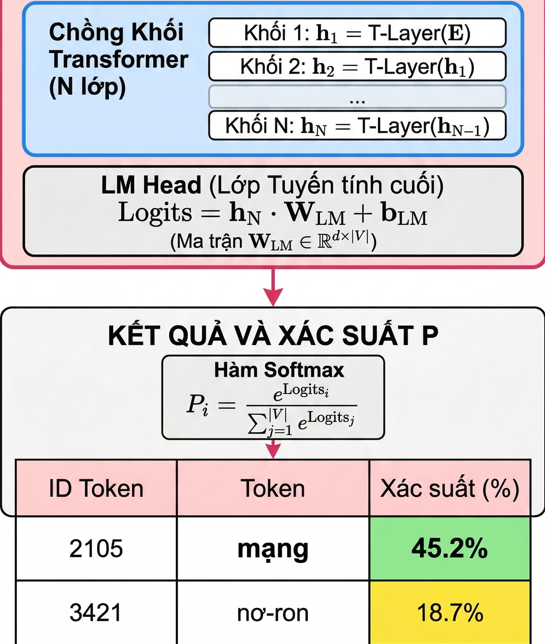
\includegraphics[width=0.7\textwidth, height=0.7\textheight, keepaspectratio]{img/minh_hoa_bo_du_doan_tu_word_predictor.png}
			\\ \vspace{0.2cm} \scriptsize{Minh họa cơ chế dự đoán từ}
		\end{column}
	\end{columns}
\end{frame}

% SLIDE 4
\begin{frame}{8.5 Cấu trúc Đầu vào}
	\begin{columns}
		\begin{column}{0.5\textwidth}
			\textbf{Luồng dữ liệu (Data Flow):}
			\begin{itemize}
				\item Tiếp nhận \textbf{vector đầu ra $h_N^L$} từ lớp Transformer cuối cùng tại token $N$.
				\item $h_N^L$ được sử dụng làm \textbf{cơ sở suy diễn} từ vựng tại vị trí \textbf{$N+1$}.
				\item \textbf{Figure 8.15} mô tả quy trình \textbf{ánh xạ} vector trạng thái ẩn $[1 \times d]$ thành \textbf{phân phối xác suất}.
			\end{itemize}
		\end{column}
		\begin{column}{0.5\textwidth}
			\centering
			% Hình tài liệu cung cấp
			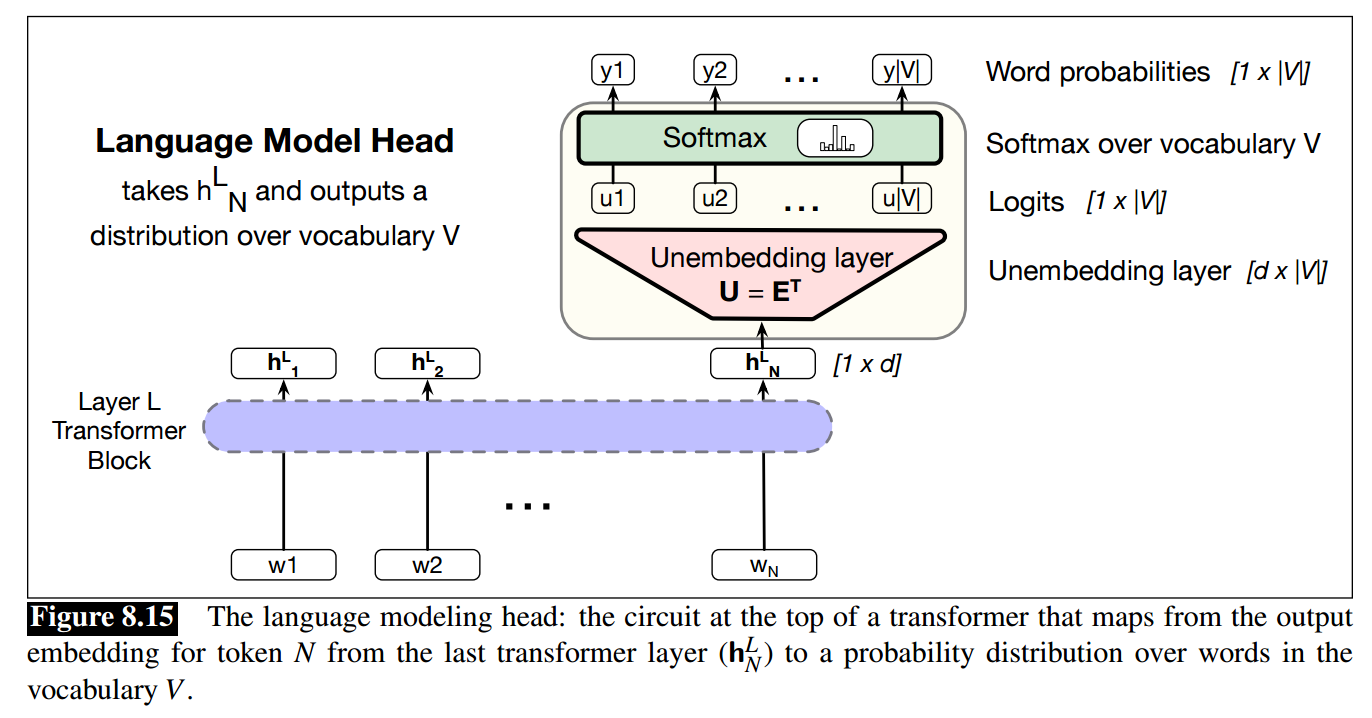
\includegraphics[width=1\textwidth, height=0.8\textheight, keepaspectratio]{img/figure8_15.png}
		\end{column}
	\end{columns}
\end{frame}

% SLIDE 5
\begin{frame}{8.5 Phép chiếu Tuyến tính và Giải nhúng}
	\begin{columns}
		\begin{column}{0.55\textwidth}
			\textbf{1. Lớp Tuyến tính (Linear Layer):}
			\begin{itemize}
				\item \textbf{Chiếu vector ẩn $h_N^L$} thành \textbf{vector logit $u$}.
				\item \textbf{Biến đổi không gian} từ $[1 \times d]$ sang \textbf{không gian từ vựng} $[1 \times |V|]$.
			\end{itemize}
			
			\vspace{0.2cm}
			\textbf{2. Kỹ thuật Weight Tying:}
			\begin{itemize}
				\item Sử dụng \textbf{ma trận chuyển vị $E^T$} làm lớp \textit{\textbf{Giải nhúng (Unembedding layer)}} để \textbf{ánh xạ ngược} về từ vựng.
			\end{itemize}
		\end{column}
		\begin{column}{0.45\textwidth}
			\centering
			% Hình placeholder tự thêm
			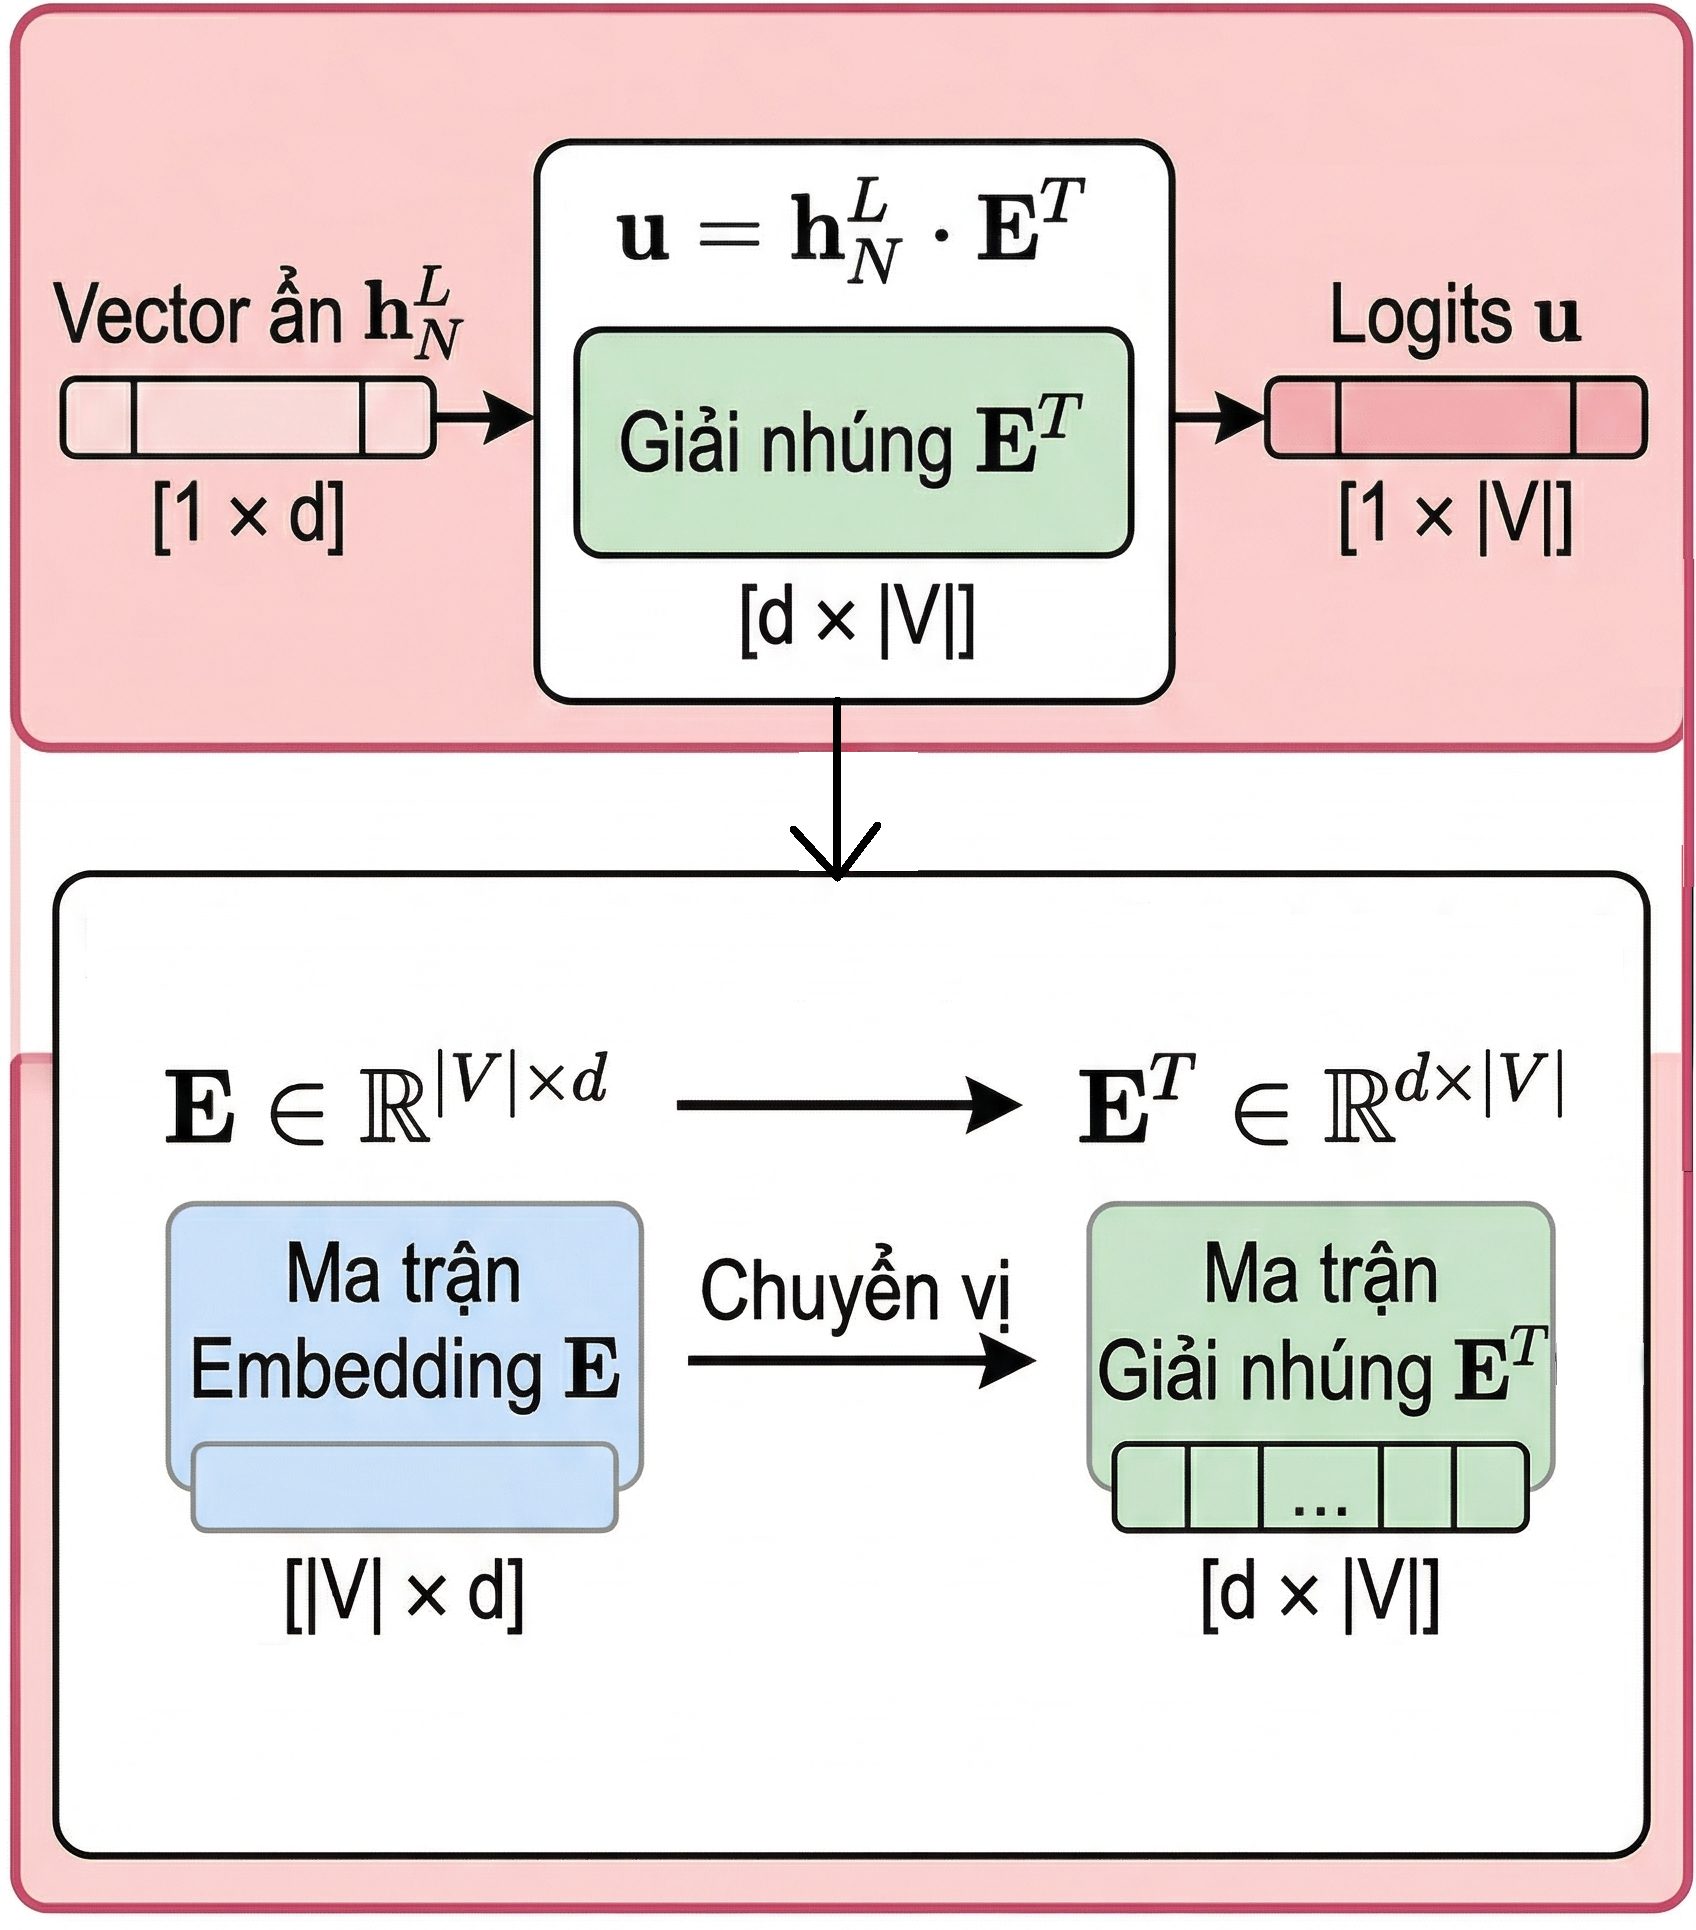
\includegraphics[width=0.8\textwidth, height=0.8\textheight, keepaspectratio]{img/minh_hoa_ma_tran_chuyen_vi_unembedding.png}
			\\ \vspace{0.2cm} \scriptsize{Ánh xạ ngược qua ma trận chuyển vị $E^T$}
		\end{column}
	\end{columns}
\end{frame}

% SLIDE 6
\begin{frame}{8.5 Chuẩn hóa Xác suất và Sinh văn bản}
	\begin{columns}
		\begin{column}{0.55\textwidth}
			\textbf{Hàm Softmax:}
			\begin{itemize}
				\item \textbf{Chuyển đổi logit $u$} thành \textbf{phân phối xác suất $y$}.
				\item Hệ phương trình cốt lõi:
				\begin{equation*}
					u = h_N^L E^T
					\tag{8.46}
				\end{equation*}
				\begin{equation*}
					y = \text{softmax}(u)
					\tag{8.47}
				\end{equation*}
			\end{itemize}
			
			\textbf{Quá trình Lấy mẫu (Sampling):}
			\begin{itemize}
				\item \textbf{Sinh văn bản} bằng cách \textbf{lấy mẫu một từ} từ phân phối $y$.
			\end{itemize}
		\end{column}
		\begin{column}{0.45\textwidth}
			\centering
			% Hình placeholder tự thêm
			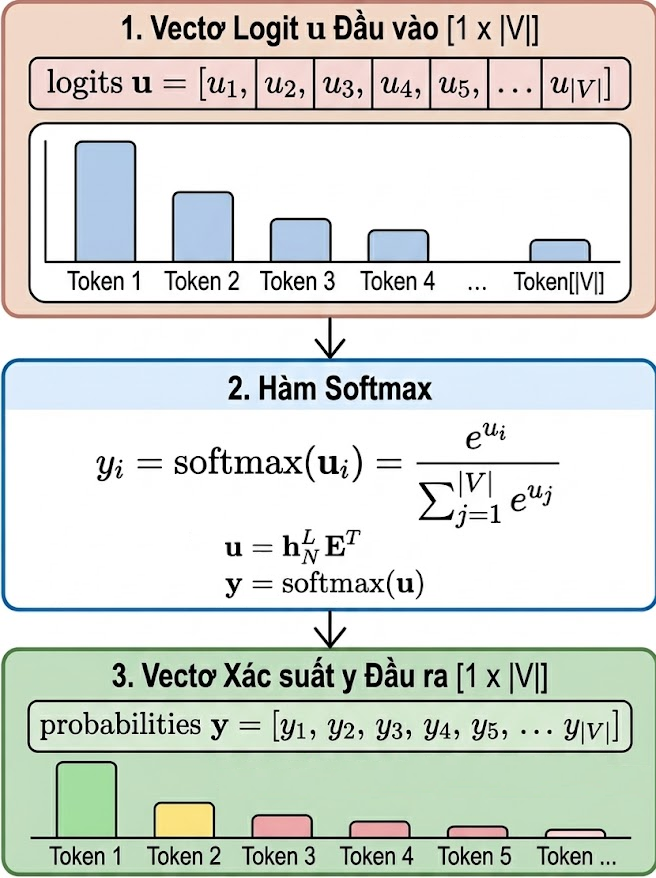
\includegraphics[width=0.8\textwidth, height=0.8\textheight, keepaspectratio]{img/minh_hoa_ham_softmax_va_lay_mau_sampling.png}
			\\ \vspace{0.2cm} \scriptsize{Từ Logit đến xác suất}
		\end{column}
	\end{columns}
\end{frame}

% SLIDE 7
\begin{frame}{8.5 Kiến trúc Decoder-Only}
	\begin{columns}
		\begin{column}{0.5\textwidth}
			\textbf{Kiến trúc Xếp chồng (Stacked Architecture):}
			\begin{itemize}
				\item Đầu vào mỗi lớp $x_i^L$ \textbf{kế thừa trực tiếp} từ đầu ra $h_i^{L-1}$ của \textbf{lớp liền trước}.
			\end{itemize}
			
			\vspace{0.2cm}
			\textbf{Thuật ngữ Decoder-Only:}
			\begin{itemize}
				\item Định danh cho các \textbf{mô hình ngôn ngữ nhân quả một chiều} (unidirectional causal).
				\item \textbf{Chỉ sử dụng cấu trúc giải mã (decoder)} so với mô hình dịch máy encoder-decoder nguyên thủy.
			\end{itemize}
		\end{column}
		\begin{column}{0.5\textwidth}
			\centering
			% Hình tài liệu cung cấp
			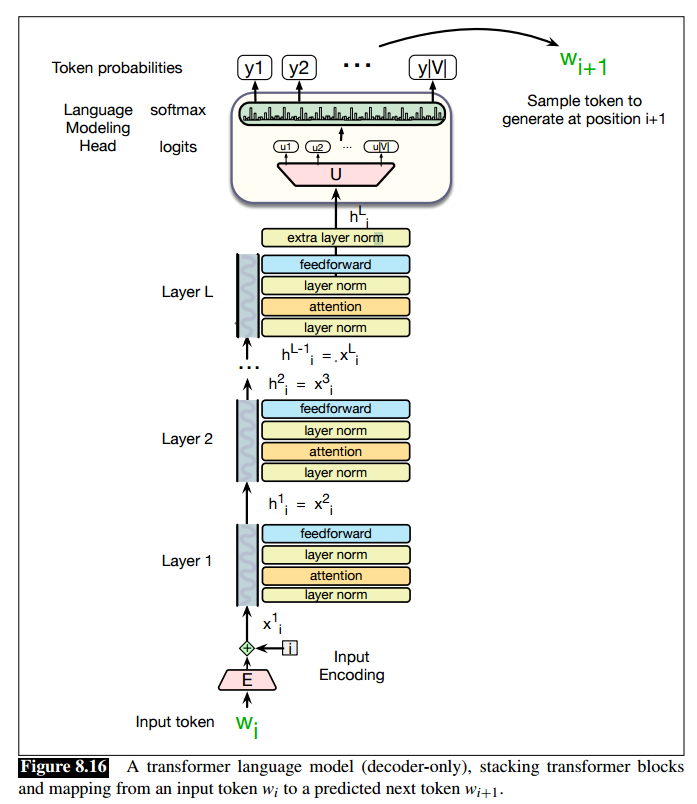
\includegraphics[width=0.95\textwidth, height=0.85\textheight, keepaspectratio]{img/figure8_16.png}
		\end{column}
	\end{columns}
\end{frame}

